% Template for ICIP-2019 paper; to be used with:
%          spconf.sty  - ICASSP/ICIP LaTeX style file, and
%          IEEEbib.bst - IEEE bibliography style file.
% --------------------------------------------------------------------------
\documentclass{article}
\usepackage{spconf,amsmath,graphicx}
% \setlength{\parskip}{0.1em}

%\parskip 0.2in %Separation between paragraphs
% Example definitions.
% --------------------
\def\x{{\mathbf x}}
\def\L{{\cal L}}

% Title.
% ------
\title{Multi-modal Medical Image Fusion Using Wavelet Techniques}
%
% Single address.
% ---------------
%\name{Author(s) Name(s)\thanks{Thanks to XYZ agency for funding.}}
%\address{Author Affiliation(s)}
%https://de.overleaf.com/project/5d8d41d85f86a90001d55d6d
% For example:
% ------------
%\address{School\\
%	Department\\
%	Address}
%
% Two addresses (uncomment and modify for two-address case).
% ----------------------------------------------------------
\twoauthors
  { Gomez Gonzalez, Juan M. \textsuperscript{1}; Hoyos Velasquez, Natalia \textsuperscript{1}; Zaki, Shadi \textsuperscript{1}; Woidelko, Mirco F. \textsuperscript{2} \sthanks{The author performed the work while at University of Waterloo}}
	{\small \textsuperscript{1} Dept. of Electrical and Computer Engineering, University of Waterloo, CA. \\
	\small \textsuperscript{2} Dept. of Mechanics and Ocean Engineering, Hamburg University of Technology, DE.}
  {}
	{}


\begin{document}
%\ninept
%
\maketitle

\begin{abstract}
\ninept
\textbf{The clinical role of medical image fusion in the assistance of accurate medical diagnostics is highly significant. As a result, extensive research has been conducted for the purpose of improving the quality as well as the information content that can be retrieved from multi-modal images. This survey discusses the strengths and limitations of various wavelet techniques that have been extensively studied and employed for the fusion of multi-modal medical images. The proposed techniques have proven successful for the purpose of fusing complementary information content of medical images, yet they still possess the limitation of edge and curve detection.} 
\end{abstract}
%
\begin{keywords}
\ninept
Discrete Wavelet Transform, Multiwavelet Transform, Dual-Tree Complex Wavelet Transform, Wavelet, Image fusion
\end{keywords}
%
\section{Introduction}
\label{sec:intro}
Digital image processing is widely used in many different areas of engineering, and an important application of it is in the field of image fusion \cite{Deshmukh.2015,Kaur.2015}. 
%In image fusion two or more images are combined or merged by means of their shared and redundant features, resulting in an image containing the common and complimentary information of the images. Thus, the newly created image is more informative than the individual images. %This attribute of image fusion makes it especially interesting for fields in which different superposed images with complementary information assist to make a more informed decision, such as in medical imaging \cite{DBLP:journals/corr/JamesD14}.
Image fusion is especially useful when images with ancillary information are available. Thereof, a more informed decision can be derived based on the combined data - the fused image. 
% \footnote{Medical imaging is the collective term for different technologies to view the human body in a non-invasive way, providing doctors with the information needed to diagnose, monitor or treat their patients.}.

Currently used imaging technology for medical purposes like magnetic resonance imaging (MRI), computerized tomography (CT), or positron emission tomography (PET) among others are limited by the type of structure or process they can observe (soft tissue, hard tissue or metabolic processes), and, thus, provide a rather narrow set of characteristic information with each technology having its practical limitations. Image fusion is a useful tool to combine these different imaging techniques, which in turn helps to overcome their respective limitations, while at the same time improving clinical accuracy and increasing the robustness of the analysis \cite{DBLP:journals/corr/JamesD14}. Image fusion can therefore be considered a tool that reduces the effort radiologists have to do in order to analyze medical images and make a diagnosis. Furthermore, fused images could potentially prevent costly post-analysis as a machine learning system would not need to compare redundant data in multiple images. Likewise, image fusion can save storage space on hospital servers as there is less redundant information to store \cite{Bhateja.2015}.

In the past decades, different methods and variations thereof have been developed and implemented in medical image fusion. They can be classified as either being in the spatial domain or in the transform domain \cite{K.Padmavathi.2016}. In the transform domain, a common method in medical image fusion is the wavelet transform, which preserves time and frequency \cite{Kaur.2015, K.Padmavathi.2016, Agarwal.2015}.
However, the wavelet transform has limitations with regard to directionality and shift-invariance \cite{Bhateja.2015, Agarwal.2015}. In recent years, new techniques based on wavelet transforms, like the Multiwavelet Transform \cite{Wang2004} and the Dual-Tree Complex Wavelet Transform (DTCWT)  \cite{K.Padmavathi.2016, Talbi.2018} have emerged. This paper presents the Discrete Wavelet Transform, some of its recent adaptations, and their advantages and limitations.


\section{Different Wavelet Techniques}
\label{sec:DiffWaveTrans}

\subsection{Discrete Wavelet Transform}
\label{sec:DWT}

The base wavelet technique that is commonly used in medical image fusion is the discrete wavelet transform (DWT). DWT is based on the idea of replacing the sinusoidal functions of the Fourier transform, which oscillate infinitely, with wavelets that consist of locally oscillating basis functions with an amplitude that begins at zero, increases, and then fades back to zero. Similarly to the Fourier transform, DWT allows the decomposition of the image in terms of different wavelets that preserve the image information. Each one of these wavelets is a modified (i.e. shifted and/or stretched) version of a fundamental band-pass wavelet function $\psi(t)$ and a low-pass scaling function $\phi(t)$, as seen in equations \ref{eq:1} to \ref{eq:3} \cite{IvanW.Selesnick.2005}.
% \begin{equation}
% x(t) = \sum_{n=-\infty}^{\infty} c(n)\phi(t-n) + \sum_{j=0}^{\infty}\sum_{n=-\infty}^{\infty} d(j, n)2^{j/2} \psi(2^{j}t-n)
% \end{equation}
\begin{align}
\begin{split}\label{eq:1}
    x(t) ={}& \sum_{n=-\infty}^{\infty} c(n)\phi(t-n)\\
         & + \sum_{j=0}^{\infty}\sum_{n=-\infty}^{\infty} d(j, n)2^{j/2} \psi(2^{j}t-n)
\end{split}\\
\begin{split}\label{eq:2}
    c(n) ={}& \int_{-\infty}^{\infty}x(t)\phi(t-n)dt
\end{split}\\
    d(j,n) ={}& 2^{j/2}\int_{-\infty}^{\infty}x(t)\psi(t)(2^jt-n)dt\label{eq:3}
\end{align}

%% For above, missing reference A wavelet based image fusion tutorial
In other words, the wavelet transform uses both shifting and scaling operations to obtain information related to the time and frequency of the signals of the image. After applying the DWT transform, sub-sampling and filtering operations are incorporated horizontally and vertically, resulting in an image divided into four sub-bands or sub-images: LL, LH, HL and HH, each with its own set of information as seen in Fig.\ref{DWT}. The labels in the figure indicate how the sub-bands were generated referring to the type of filtering performed across the image columns and rows, respectively. The LL sub-band can be considered as a smoothed as well as sub-sampled version of the original that contains the average information, whereas the other sub-bands contain details of horizontal, vertical and diagonal directional information. In the higher bands, a higher absolute value of the coefficients represents features such as lines or edges \cite{M.Haribabu.2017, Pajares.Delacruz.2004}.

    \begin{figure}[hbt!]
        \centering
        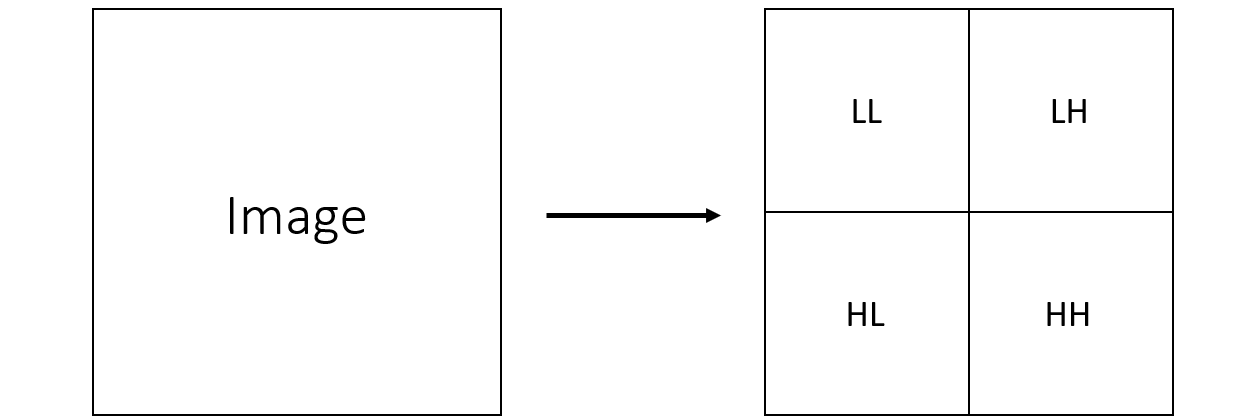
\includegraphics[width=\linewidth]{Img/DWT.png}
        \caption{ Discrete Wavelet Transform. Adapted from \cite{Chiorean.Vaida.2009}.}
        \label{DWT}
    \end{figure}

For image fusion, the same process can be performed on different annotated and aligned images to obtain the wavelet coefficients. It is fundamental that the images are adequately aligned and registered before combining to prevent the appearance of edge artifacts. Coefficient pairs of corresponding resolution levels, frequencies and representations are merged together with the guidance of a fusion rule. There are many rules for image fusion, and they can be dependent on the application and on the sub-band to be fused. Some of the rules are very straightforward, like selecting the minimum, maximum or mean values of the transform coefficients. Others are more complex operations that use spatial filtering, like the energy filter or the Laplacian edge filter. \cite{Pajares.Delacruz.2004, Chiorean.Vaida.2009}

Once the coefficients are consolidated, the final step in the fusion process is to reconstruct an image from the decomposed fused image data by employing the inverse discrete wavelets transform (IDWT), where the information in the combined coefficients is also conserved \cite{Wang2004, Pajares.Delacruz.2004, Liu2010, Peng2015}.

\subsubsection{Advantages of DWT}
The limited duration of the wavelets is the primary advantage of the wavelet transform over the Fourier transform, as it provides more resolution in the time domain \cite{Gonzalez.Woods.2008}. The irregularity and enhanced temporal resolution of DWT provides an effective representation for many types of signals that are not well matched by the Fourier basis, which in general envisions a periodic signal. Particularly, since wavelets oscillate locally, they are a better basis for analysis of signals with discontinuities, jumps or spikes, as only wavelets overlapping the singularity would have a large wavelet coefficient while the rest of the coefficients would be small \cite{IvanW.Selesnick.2005, Cheng.He.Lv.2008}. 

Furthermore, due to the nature of DWT, it allows for the multi-resolution analysis of an image. This in turn means that the features of an image can be analyzed in multiple scales and, thus, have a better understanding of the inherent components of the image \cite{Chiorean.Vaida.2009, Cheng.He.Lv.2008, Kavitha.Chellamuthu.Rajesh.2012}.

\subsubsection{Limitations}
In the past, DWT was limited by its computational complexity in implementation. This was solved in 1989 when Stephane Mallat developed a computationally efficient algorithm for DWT, akin to what was achieved with the Fast Fourier Transform \cite{Gonzalez.Woods.2008, Mallat.1989}. This algorithm allowed for the development of the Fast Wavelet Transform, which in turn permitted the adoption of the DWT for common processes and practices.

One of the main limitations of DWT in the present is that it is susceptible to shift variance. This means that a small shift in the signal will generate a marked perturbation of the wavelet coefficient oscillation pattern \cite{IvanW.Selesnick.2005}. Apart from this, there is also a problem with aliasing. Due to the fact that the coefficients are calculated by down-sampling operations with non-ideal high-pass and low-pass filters, a dramatic aliasing effect can be present in the image if any kind of processing is done in the wavelet coefficients \cite{IvanW.Selesnick.2005}. Additionally, Another limitation is present in the form of a lack of directionality. Ridges and edges are hard to model and process because the tensor product construction of the wavelets creates a checkerboard pattern oriented in multiple different directions, a problem not present in the case of higher dimension Fourier sinusoids \cite{IvanW.Selesnick.2005}.

\subsection{Multiwavelet Transform}
Another wavelet technique that is commonly used with great success in medical multi-modality fusion is the multiwavelet transform. Multiwavelets are an extension of scalar wavelets. In fact, scalar wavelets can be considered a special case of multiwavelets with a matrix filter bank size of $1 \times 1$ ($r = 1$) \cite{Wang2004}. Multiwavelets are very similar to scalar wavelets, but they have unique desirable properties that make them more attractive to researchers, particularly in the field of medical image fusion \cite{Wang2004, Liu2010, Peng2015}.

Unlike scalar wavelets, which only have one associated scaling function, $\phi(t)$, and one associated wavelet function, $\psi(t)$, multiwavelets can have an arbitrary number of scaling and wavelet functions ($r > 1$). The set of scaling functions, referred to as the multiscaling function, is denoted by $\Phi(t)$. Similarly, the set of wavelet functions is denoted by $\Psi(t)$, and is referred to as the multiwavelet function. Furthermore, the multiscaling and multiwavelet functions can be described, respectively, by equations \ref{eq:4} and \ref{eq:5} \cite{Wang2004}:

\begin{gather}\label{eq:4}
 \Phi(t) = [\phi_1(t)\; \phi_2(t)\;...\;\phi_r(t)]^T = \sum_{k=0}^{m-1} G_k \Phi(2t-k) \\\label{eq:5}
  \Psi(t) = [\psi_1(t)\; \psi_2(t)\;...\;\psi_r(t)]^T = \sum_{k=0}^{m-1} H_k \Phi(2t-k)
\end{gather}

In these equations, $G_k$ and $H_k$ are $r \times r$ low and high pass filters for each $k$, respectively, and $m$ is the number of scaling coefficients. Although $r$ can be arbitrarily large, this paper will focus only on a subset of multiwavelets with $r = 2$, since they have been extensively studied and used in fusion of multi-modal medical images.
Using multiwavelet transform decomposition requires the input signal to be firstly preprocessed or vectorized in order to generate multiple input streams from a source stream \cite{Wang2004, Liu2010}. This stage is also referred to as the prefiltering stage, and is not needed when using scalar wavelet decomposition.
After prefiltering, and similarly to scalar wavelet decomposition, the two-dimensional image data is decomposed into sub-bands representing high and low pass filtering across two dimensions. However, unlike scalar wavelets, which base the decomposition on one set of high/low pass coefficients, multiwavelets use $r$ sets of coefficients \cite{Wang2004}.

    \begin{figure}[hbt!]
        \centering
        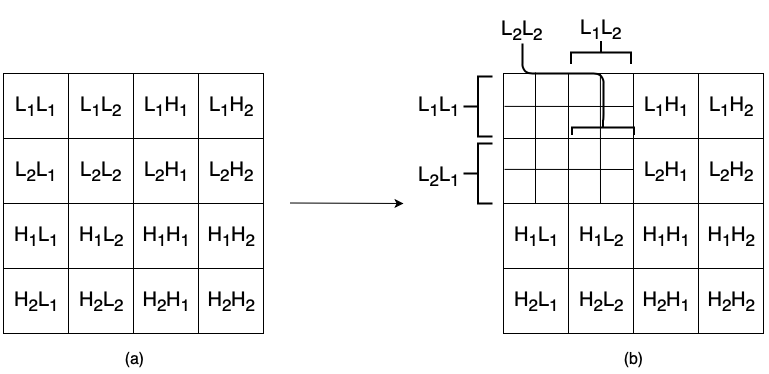
\includegraphics[width=\linewidth]{Img/Multiwavelet.png}
        \caption{(a) Single-Level Multiwavelet Decomposition with $r = 2$. (b) Two-Level Multiwavelet Decomposition. Adapted from \cite{Wang2004}}
        \label{multiwavelet}
    \end{figure}

Fig.\ref{multiwavelet}(a) illustrates the sub-bands generated by a single-level multiwavelet decomposition with $r = 2$. The subscripts indicate which set of wavelet coefficients is used. In practice, multiple levels of decomposition are performed specifically on the low-pass data \cite{Wang2004, Liu2010}, further reducing the number of low-pass coefficients, as illustrated in Fig.\ref{multiwavelet}(b). This is mainly due to the fact that most of the signal energy in natural images are in low frequency sub-bands, so multiple-level decomposition results in better energy compaction.
After image data is decomposed into multiple frequency sub-bands, one or more fusion rules are usually employed to fuse the image data based on the particular algorithm. A general fusion rule is selecting the larger absolute value of the two images' multiwavelet coefficients pixel-by-pixel \cite{Wang2004}. This works because larger absolute coefficients usually correspond to sharper brightness changes in images, and, thus, to dominant image features such as edges and boundaries. However, relevant image features almost always span multiple pixels. As a result, alternative approaches have been explored. For example, \cite{Wang2004} uses different rules for lower and higher frequency sub-bands. The average of wavelet coefficients is taken as a fusion rule for lower frequency sub-bands, since low frequencies in images represent their rough features. In higher frequency sub-bands, a pattern contrast-based measure is employed for pixel selection. Moreover, \cite{Liu2010} evaluated the results obtained using different fusion rules. In lower frequency sub-bands, they evaluated a weighted average method and a gradient method. On the other hand, in the higher frequency sub-bands, they evaluated maximum fusion, a contrast-based fusion rule, and classification fusion. Finally, \cite{Liu2010} concluded that using the gradient method for low frequencies along with the classification fusion for higher frequencies lead to a more appropriate fusion effect.

Finally an image has to be reconstructed from the decomposed fused image data, which can be done by reversing the decomposition steps applied before fusion \cite{Wang2004, Liu2010, Peng2015}. Postfiltering is also required to revert a vector image to scalar one.

\subsubsection{Advantages of Multiwavelet Transform}
Multiwavelets possess many desirable properties that cannot otherwise simultaneously exist when using scalar wavelets. Multiwavelets can be orthogonal while simultaneously use symmetric filters \cite{Wang2004, Liu2010, Peng2015}, both considered desired transform properties. Orthogonality is important for a simple design and implementation of the transform since it allows for simpler mathematical derivations. Symmetric filters, on the other hand, are required for symmetric signal extension \cite{Wang2004}. In addition to orthogonality and symmetry, multiwavelets allow for better coding through higher order approximations, while having shorter scaling function support, which allows for more accurate localized approximations \cite{Wang2004, Liu2010}.

\subsubsection{Limitations}
One of the main limitations in multiwavelet transform is its computational complexity, particularly with multiple levels of decomposition. In fact, increasing the levels of decomposition increases the size of the top subimages exponentially, which, in turn, increases the computational workload. Another limitation of multiwavelet transform is the prefiltering stage, since choosing inappropriate prefilters can negatively influence the wavelet decomposition process.

\subsection{Dual-Tree Complex Wavelet Transform}
Dual-Tree Complex Wavelet Transform (DTCWT) can also be used for medical image fusion. Particularly, DTCWT has been used to fuse MRI/CT, MRI/Proton Density, MRI/PET, and MRI/SPECT. The main difference in the application of DTCWT for image fusion is the process of determining the coefficients for the wavelet transform \cite{K.Padmavathi.2016, Talbi.2018}. DTCWT is inspired by the Fourier transform, which, unlike DWT, has a smooth envelope, is shift invariant, has no aliasing, and is highly directional. To achieve these criteria, the wavelet function $\Psi(t)$ must be an analytic signal. Hence, it must have a real and imaginary part - which ideally are a Hilbert transform pair - 90$^{\circ}$ out of phase. To determine the real and imaginary part, two real DWTs are used in parallel. One determines the imaginary, the other determines the real valued coefficients. Each set of filters satisfies the perfect reconstruction criteria, and the filters are designed such that $\Psi(t) = \Psi_1(t)+j\Psi_2(t)$ is approximately analytic \cite{IvanW.Selesnick.2005}. Thereof, the coefficients $d(j,n)$ for the wavelets can be determined as seen in equation \ref{eq:6}.

 \begin{gather}\label{eq:6}
      2^{j/2}\Psi(2^j t-n) \longrightarrow d(j,n) = d_r(j,n)+jd_i(j,n)
 \end{gather}
 
After having processed each image through the forward transform, as described above, and having determined the low and high frequency components of the real and imaginary coefficients, the coefficients are fused based on the proposed rule.
In \cite{K.Padmavathi.2016}, a fusion rule using Principal Component Analysis (PCA) is proposed. PCA removes redundant information and computes a normalized eigenvector, which contains the weights used on the decomposed input images. Other fusion approaches for DTCWT use separate rules for high and low frequency components \cite{Talbi.2018, Xiaozhu.27.07.201529.07.2015}. Threshold fusion rules are also used together with DTCWT. The coefficients with low values are discarded and high coefficients are selected based on a varying threshold scheme to reduce noise in the fused image \cite{Srivastava.2016}. 
The fused coefficients are the input to the inverse DTCWT. As a result of the inverse DTCWT, two real value signals - one from the imaginary and one from the real valued part- are produced. These are averaged and form the fused image \cite{Talbi.2018}.

 \subsubsection{Advantages of DTCWT}
 \label{ADV_DTCWT}
The use of DTCWT has multiple advantages compared to other methods. In comparison to DWT, DTCWT produces almost analytic wavelets due to the approximately Hilbert transform pair. Hence, the drawbacks of DWT are almost fully eliminated. DTCWT is approximately shift-invariant, which reduces the ringing effect in fused images \cite{Talbi.2018}. Also, DTCWT conserves subtle texture regions and details better than DWT due to being able to differentiate between positive and negative edges\cite{Talbi.2018}. Moreover, the split into real and imaginary part causes the DTCWT to only support one frequency axis, and thus only one quadrant in a 2-D wavelet is supported. This prevents checkerboard patterns in 2-D plane and makes DTCWT directionally selective in two or more dimensions \cite{K.Padmavathi.2016}. Likewise, information about the phase is preserved in the complex valued wavelet of DTCWT \cite{K.Padmavathi.2016, Talbi.2018, IvanW.Selesnick.2005}.
Considering a perfectly shift-invariant DWT, the results of DTCWT are more desirable and achieved with a lower redundancy \cite{Talbi.2018, IvanW.Selesnick.2005}.
In comparison to other new methods, DTCWT profits from the use of two independent DWTs, since it can resort from the well-tested and optimized software and hardware used for DWT. Overall, DTCWT in medical image fusion shows top results throughout the different measures used to evaluate fused images when compared to wavelet transforms and other techniques \cite{Srivastava.2016, Goel.2017}.

\subsubsection{Limitations}
Due to its analytic property, DTCWT has overcome the limitations of DWT. Yet, the demand for approximate analytic behavior introduces high requirements for the design of the filter banks, e.g. succeeding stage filters must be different and filter banks must have an interlace property \cite{IvanW.Selesnick.2005}. Hence, the design of an appropriate DTCWT is time intensive. For image fusion, the presented form using DWT resources is not optimal for natural images, since it is inefficient to determine lines and curves from them \cite{IvanW.Selesnick.2005}. Thus, a better line and curve representation can only be achieved by using e.g. complex filter banks \cite{IvanW.Selesnick.2005}, which then cannot make use of existing software and hardware.  

\section{Conclusion}
\label{sec:print}

Medical image fusion is a still developing technique that has greatly benefited both those that work in the medical field as well as their patients. Compared with other techniques, the use of DWT has allowed for a more fine tuned adaptation to the characteristics present in medical images, e.g. a high spatial and frequency resolution.

%For base level image fusion, DWT is sufficient yet for a higher sophistication and for images with more detail the other methods need to be used.

Nonetheless, shortcomings like shift variance, aliasing and a lack of directionality have created the need to keep improving the technique. Approaches like multiwavelet transform and Dual-Tree Complex wavelet transform have addressed this limitation. Multiwavelet transform has allowed for a larger accuracy thanks to its higher order approximation, as well as having the capacity of simultaneous orthogonality and filter symmetry. DTCWT allows for the removal of the shift variance sensitivity and the lack of directionality of DWT. 
DWT can then be considered the baseline approach for medical image fusion. However, if the purpose is to preserve a higher amount of detail and texture information in the image, a more complex approach like DTCWT or multiwavelet should be used, albeit at a higher computational cost.
%On the down side, the new methods are more computing intensive.

However, edge and curve detection in medical images remains critical despite the development of DWT techniques. Further research is needed to reduce the computation cost, as well as improve processing of edges and curves for finer feature representation. This would further improve the visualization of finer details in diagnostic processes. 

% Below is an example of how to insert images. Delete the ``\vspace'' line,
% uncomment the preceding line ``\centerline...'' and replace ``imageX.ps''
% with a suitable PostScript file name.
% -------------------------------------------------------------------------
\iffalse
\begin{figure}[htb]

\begin{minipage}[b]{1.0\linewidth}
  \centering
  %\centerline{\includegraphics[width=8.5cm]{image1}}
%  \vspace{2.0cm}
  \centerline{(a) Result 1}\medskip
\end{minipage}
%
\begin{minipage}[b]{.48\linewidth}
  \centering
 % \centerline{\includegraphics[width=4.0cm]{image3}}
%  \vspace{1.5cm}
  \centerline{(b) Results 3}\medskip
\end{minipage}
\hfill
\begin{minipage}[b]{0.48\linewidth}
  \centering
  \centerline{}
%  \vspace{1.5cm}
  \centerline{(c) Result 4}\medskip
\end{minipage}
%
\caption{Example of placing a figure with experimental results.}
\label{fig:res}
%
\end{figure}
\fi




% References should be produced using the bibtex program from suitable
% BiBTeX files (here: strings, refs, manuals). The IEEEbib.bst bibliography
% style file from IEEE produces unsorted bibliography list.
% -------------------------------------------------------------------------
\bibliographystyle{IEEEbib}
\bibliography{strings,refs}

\end{document}
